\documentclass[main.tex]{subfiles}
\begin{document}
\chapter{Le cancer~: aspects biologique et clinique.}\todo[noline]{tumeur en general ou GIST?}
\mylettrine{L}{a} biologie du cancer est encore à ce jour non entièrement connue. Sa complexité n'étant pas des moindres, on présentera dans ce chapitre uniquement les points clés nécéssaire à l'élaboration des modèles mathématiques présentés dans ce manuscrit. On présentera tout d'abord sommairement comment croît une tumeur, puis comment elle se répand dans l'organisme. Nous aborderons ensuite les traitements actuels. Enfin, nous examinerons de plus près le fonctionnement d'un scanner; les scanners constituant la seule et unique information médicale dont nous disposons. 

\section{Croissance tumorale}
%\todo[noline]{La tumeur en grandissant, va pousser vers l'extérieur le réseau sanguin qui l'alimente ! (La tumeur exerçant une pression sur celui-ci) --> valable que pour les méta, tumeur primit = infiltrante}
Une tumeur est un ensemble de cellules de l'organisme se multipliant de manière dégénérée. Certains scientifiques s'accordent à dire que cela partirait d'une seule cellule (pour l'instant aucune preuve de cela n'a encore été apportée~: le sujet reste ouvert). Chaque cellule fille est alors à son tour dégénérée et se multiplie encore et encore. La tumeur pourrait alors grandir exponentiellement. En réalité, la croissance tumorale est limitée par les besoins de glucose et d'oxygène. En effet, à force de se multiplier les cellules sont en surpopulation. Les nutriments et l'oxygène viennent à manquer : c'est l'\emph{hypoxie}. Les cellules du bord de la tumeur consomment tout et n'en laissent pas assez pour celles situées plus au centre. C'est dans ces cas là que l'on peut voir sur les scanners des tumeurs avec 2 nuances de gris~:
\begin{itemize}
\item un gris foncé au centre, emplacement du tissu en partie nécrosé
\item un gris plus clair sur le pourtour, lieu de la prolifération
\end{itemize}

\newpage
\begin{wrapfigure}[18]{R}{.5\textwidth}
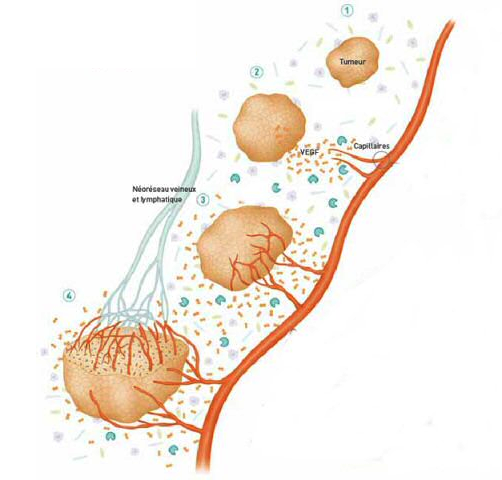
\includegraphics[width=.5\textwidth]{schema/angiogenese.jpg}
\captionof{figure}{\label{fig:schema_angio} Schéma descriptif de l'angiogénèse générant la néovascularisation \cite{web1}.}
\end{wrapfigure}
Les cellules en hypoxie vont alors entrer dans un état de quiescence et vont sécréter des \emph{facteurs de croissance}, dont le VEGF (Vascular Endothelial Growth Factor). Ces protéïnes commandent la création de nouveaux vaisseaux sanguins, processus appellé \emph{angiogenèse}. Les cellules endothéliales, cellules qui recouvrent la paroi intérieure des vaisseaux sanguins et destinataires de ces facteurs de croissance, vont alors construirent des nouveaux vaisseaux sanguins par chimiotactisme c-à-d que les nouveaux vaisseaux sanguins sont orientés dans le sens où la concentration de facteur de croissance est la plus forte. Ainsi la tumeur se créée son propre réseau sanguin~: la \emph{néovascularisation}. La nourriture et l'oxygène redeviennent de nouveau abondants. 
Les cellules qui étaient en hypoxie vont alors se remettre à proliférer jusqu'à ce que de nouveau, il y ait surpopulation. Et ainsi de suite, le cycle continue. On peut visualiser ce cycle sur le schéma présenter Figure~\ref{fig:schema_angio}. Notez qu'une cellule saine n'est en général jamais quiescente~: si les conditions extérieures ne sont pas bonnes (surpopulation, manque de nutriments, etc ...), elle va activer son auto-destruction~: c'est l'\emph{apoptose}. A cause de mutation, les cellules cancéreuses sont nettement moins (voire pas) sensible à ce mécanisme. 

\section{Dissémination des métastases}
\begin{wrapfigure}[17]{l}{.5\textwidth} %%% L : Left flottant / l: left non flottant (pas de pagebreak)
\setlength{\unitlength}{.005\textwidth}
\vspace{-9mm}
\begin{picture}(100,93)
\tiny 
\put(0,2){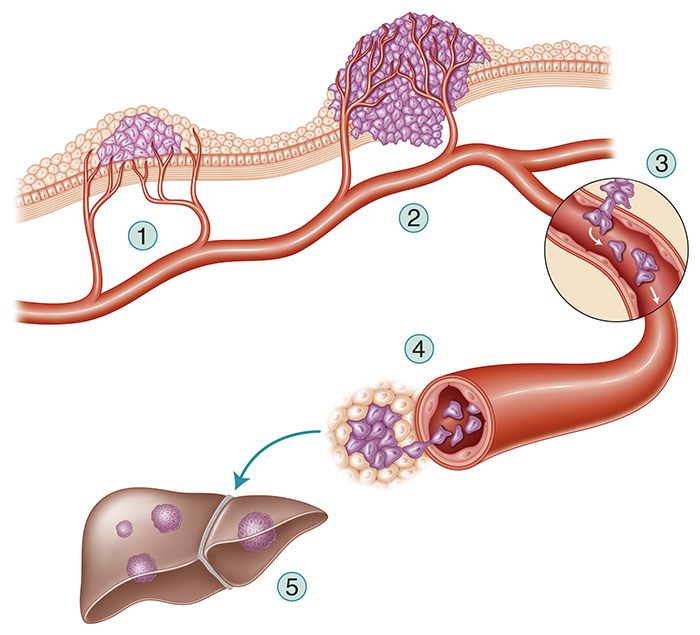
\includegraphics[width=.5\textwidth]{schema/cellules_tumorales_circulantes_copyright.jpg}}
\put(30,0){Copyright Eléonore Lamoglia/Institut Curie}
%%\put(0,0){\rect{0}{0}{100}{93}}
\end{picture}
\captionof{figure}{\label{fig:schema_dissemination_metastase} Dissémination des métastases.}
\end{wrapfigure}
L'ensemble du processus métastatique est résumé sur le schéma présenté Figure~\ref{fig:schema_dissemination_metastase}. Décrivons le. La tumeur primaire  cherche continuement à se vasculariser toujours plus, mais paradoxalement, sa croissance va endommager le réseau sanguin qui l'irrigue. Une partie des cellules tumorales (cellules invasives) va alors pouvoir pénétrer dans les voies sanguines. La plupart de ces essaims seront éliminés par le système immunitaire. Une partie arrivera à s'installer dans un autre organe~: elle forme des tumeurs filles appelées~\emph{métastases}. 

De simple cellules ne pourraient pas nicher dans un autre organe que celui auquel elles appartenaient au départ. Les cellules tumorales le peuvent, car à force de division elles s'indifférencient. C'est-à-dire qu'elles s'approchent de ce qu'elles étaient au stade embreyonnaire~: des cellules souches qui en se différenciant formeront aussi bien des cellules de l'intestin que des cellules du foie. Ce type de cellules, bien que provenant de l'intestin, n'est donc pas reconnu comme étranger au foie et la métastase peut s'installer. La métastase créera ensuite son réseau néovasculaire tout comme une tumeur primaire.

\section{Les traitements}
A l'heure actuelle aucun traitement ne permet de guérir de manière sûre les cancers, d'autant plus s'ils sont avancés.  Cependant plusieurs techniques existent pour prolonger et/ou améliorer la vie des patients.
\paragraph{La chirurgie} ne peut-être réalisée que sur des cancers primaires, non métastasés et donc détectés tôt. C'est la première option considérée par le corps médical (bien que la chirurgie elle-même puisse être source de dissémination de métastase, \cf par exemple  \url{http://www.sciencedirect.com/science/article/pii/S0748798305000089}).

\paragraph{L'ablation par radiofréquence} permet, à l'aide d'une sonde électromagnétique à haute fréquence, de bruler une région définie par le médecin. On peut ainsi réaliser une ablation sans avoir à opérer le patient. Cette technique  
ne peut cependant être utilisée que pour de petite tumeur, ne dépassant pas une certaine taille (de l'ordre du centimètre \todo{A verif, ref?}) et n'étant pas à proximité d'organes sensibles. 

\paragraph{La radiothérapie} consiste à irradier une zone de l'organisme par une forte dose de rayons X. Ceci a pour effet de détruire les cellules qui se multiplient, et donc par voie de conséquence, les cellules cancéreuses. Cette méthode présente les mêmes limitations que la radiofréquence à savoir que son efficacité est limité à des petites tumeurs. La radiothérapie est souvent utilisé à titre paliatif sur des petites métastases (pulmonaires notamment).

\paragraph{La chimiothérapie} est un médicamment \emph{cytotoxique} (\ie qui détruit les cellules) administré en intraveineuse. Elle est suffisament petite pour pénétrer à l'intérieur des cellules. Elle agit sur toutes les cellules en division trop rapide en affectant soit directement la mitose, soit la duplication de l'ADN. Ceci explique ses principaux effets secondaires car elle va impacter aussi sur des cellules saines à division naturellement rapide comme les cellules responsables de la pousse des cheveux, les cellules intestinales (de l'épithélium), les cellules sanguines (à l'origine d'affaiblissement du système immunitaire et d'anémies notamment) ou encore les gamètes.

\todo[noline]{section RECIST ?}
\paragraph{Les thérapies ciblées} sont également des médicamments administrés par voies intraveineuses. Bien qu'étant diffusées dans tout l'organisme, ces thérapies  ciblent un type spécifique de voie moléculaire (ou de récepteur), voie moléculaire généralement caratéristique des cellules malignes. Ce peut-être des anticorps (X-mab) ou bien de petites molécules ciblant les fonctions tyrosine kinase (X-inib), fonctions impliquées dans l'activité cellulaire et la mitose. 

En exemple on pourra citer l'\emph{imatinib} (Glivec) qui se fixe sur les récepteurs cellulaires (récepteurs de tyrosine kinase, RTK) commandant l'activité intra cellulaire. En inhibant ces récepteurs, l'apoptose tends à se réactiver dans les cellules défectuesues. On peut également citer le \emph{bevacizumab} (Avastin), qui inhibe l'angiogenèse, en se fixant sur les récepteurs de VEGF. D'autres molécules, comme  le sorafenib ou le sunitinib, ont des effets multiples. 
Le \emph{sorafenib} (Nexavar) est un inhibiteur, à la fois, de VEGFR et de Raf-kinase (tyrosine kinase intervenant dans la cascade de kinases activées lors de la mitose). 
Le \emph{sunitinib} (Sutent) inhibe également les VEGFRs ainsi que les KIT-kinases (protéïne CD117, qui est une tyrosine kinase très souvent exprimées dans le cas de GIST, kinases normalement produites uniquement par les cellules souches).
\todo[noline]{Kit --> commande la survie, la prolif, ou la division cellulaire}


Tous les cas cliniques que nous étudions dans cet ouvrage ont été traités avec ce type de traitement. Dans le cas de métastases de GIST, l'imatinib est recommandé en première ligne. Si celui-ci devient inefficace (ce qui arrive très souvent, des cellules résistantes se développant), le sunitinb est utilisé en seconde ligne. (REF)\todo[noline]{\url{http://www.sciencedirect.com/science/article/pii/S0140673606694464}}
\todo[noline]{\url{http://jco.ascopubs.org/content/25/30/4793.short}}
Dans certains cas de mutation génétique (du gène KIT notamment), il a même été montrer une résistance à l'imatinib plus accrue que chez les autres patients [???].

%============= deb rapportstage M2 ==============\\
%
%\subsubsection{La chimiothérapie}
%La chimiothérapie est l'injection dans le sang d'une substance chimique modifiant la forme de l'ADN de l'ensemble des cellules de l'organisme. Ceci a pour effet que toute cellule voulant se diviser péri. Ceci permet de limiter donc la croissance de la tumeur. Cependant le traitement agit sur toutes les cellules, et donc sur les cellules saines également. Ce qui n'est pas sans laissé d'effets secondaires. L'organisme ne peut plus fabriquer de nouvelle cellules là où il y en a besoin, ce qui se traduit par la perte des cheveux, etc \ldots
%
%\subsubsection{Les anti-angiogéniques}\label{trait antiangio}
%Les anti-angiogénique sont des molécules inhibitrices de l'angiogenèse. Les antiangiogéniques peuvent être classés , selon leur mode d'action, en deux catégories :
%\begin{enumerate}
%\item Les protéïnes se placent sur les récepteurs spécifiques à la VEGF sur les cellules endothéliales, inhibant ainsi l'effet de la VEGF.
%\item Ou bien elles se placent directement sur la VEGF, l'empêchant ainsi de se fixer aux cellules endothéliales.
%\end{enumerate}
% En administrant des anti-angiogénique au patient, on prive alors l'organisme de la création de nouveaux vaisseaux sanguins. La tumeur ne peut alors plus s'alimenter. Ceci n'est pas non plus sans effet secondaires : difficultés de cicatrisation par exemple. Les anti-angiogéniques ont pour effet également de renforcer le réseau sanguin existant. Ceci limite donc la dissémination des métastases par voie sanguine, car celles-ci ont beaucoup plus de mal à entrer dans le réseau.
%
%\subsection{Chimiothérapie et anti-angiogéniques}
%Il s'avère qu'une chimiothérapie seule est assez inefficace. En effet, en grandissant la tumeur détériore le réseau sanguin qui l'alimente. Le traitement arrivant par voie sanguine n'a donc aucune chance d'atteindre le centre de la tumeur. En cumulant chimiothérapie et anti-angiogéniques, le réseau sanguin est consolidé et nettement moins endommagé par la tumeur ce qui permet à la chimiothérapie d'atteindre le coeur de la tumeur et ainsi agir de manière efficace.\\
%=============   FIN RAPPORT STAGE M1  ===========\\

\section{Fonctionnement du scanner}
\subsection{Le scanner en général}
Le scanner est un examen médicale qui permet d'acquérir des images d'une partie de l'organisme par le biais d'une irradiation aux Rayons~X. Oui, oui, une irradiation ! Cependant l'irradiation est faible et de plus en plus d'études mettent en avant des méthodes pour la réduire  \url{http://www.ncbi.nlm.nih.gov/pmc/articles/PMC2743386/} ). Le bénéfice est donc très important devant les risques marginaux. C'est certainement l'une des raisons pour laquelle le scanner (tout comme la radio, ou l'IRM) est aujourd'hui très utilisé pour diagnostiquer une maladie, ou ne serait-ce même que pour contrôler la santé d'un patient.


\begin{wrapfigure}[18]{r}{.3\textwidth} %%% L : Left flottant / l: left non flottant (pas de pagebreak)
\vspace{-5mm}
\setlength{\unitlength}{.0032\textwidth}
\begin{picture}(100,121)
\scriptsize
%\footnotesize
\put(0,0){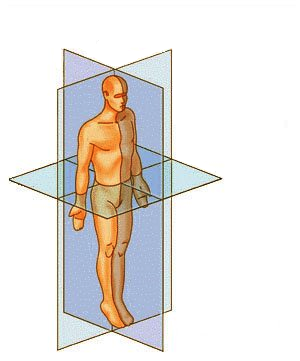
\includegraphics[width=.32\textwidth]{schema/Coupe_anatomie.jpg}}
\put(37,113){\vector(-1,-1){10}}
\put(69,100){\vector(-1,-1){10}}
\put(75,46){\vector(-1,1){10}}
\put(0,115){Plan sagital (ou frontal)}
\put(71,102){Plan}
\put(71,95){coronal}
\put(72,39){Plan}
\put(66,32){axial (ou}
\put(64,25){transverse)}
%%\put(100,0){\line(0,1){121}}
\end{picture}
\captionof{figure}{\label{fig:schema_coupe} Plans de coupe du corps humain.}
\end{wrapfigure}
Un scanner procède par acquisition d'images en couches. En ce qui concerne le scanner du thorax, le patient est \og découpé \fg{} de part en part 
\url{http://www.impactscan.org/download/msctdose.pdf} selon le plan axial. 
Sur chacun de ces plans on mesure l'absorption aux rayons~X~: la \emph{tomodensitométrie}. Cette absorption dépend de la densité du tissu mais pas seulement~: elle dépend aussi de sa nature. 
Chaque constituant de l'organisme à sa propre tomodensimétrie. La tomodensimétrie se mesure en \emph{unité Hounsfield}~(HU). Sur cette échelle, l'absorption au Rayons~X de l'eau est définie comme étant zéro. Toute autre tomodensimétrie est alors exprimée relativement à cette absorption de référence. Par exemple l'air a une tomodensimétrie de -1\,000\,HU, le poumon de -500\,HU, la graisse de -100 à -50\,HU, le foie autour de 50\,HU, les os entre +700 et +3\,000\,HU selon s'ils sont spongieux ou non. La tomodensimétrie est donc très variable. Pour pouvoir visualiser cette quantité, il est nécessaire de choisir une échelle adaptée à ce que l'on veut regarder. L'échelle sera défini par~:
\begin{itemize}
\item deux absorptions limites que l'on choisi. Le noir est associé à la plus petites de ces bornes, le blanc à l'autre. Au delà de ces bornes aucune nuance de couleur n'apparaitra.
\item une fonction qui va définir la manière dont on passe du noir au blanc. Généralement, une fonction linéaire est considéree c-à-d que la variation du noir au blanc est constante.
\end{itemize}
Par exemple, si l'on s'intéresse aux poumons, on pourra fixer l'échelle entre -1\,200 et 200\,HU (qui est l'échelle sugérée par le logiciel OsiriX dans le cas du poumon). Avec cette échelle le foie apparait tout blanc avec très peu de nuances. Elle donc inadaptée si l'on souhaite observer le foie~! Pour le foie, une échelle allant de -135 à +215\,HU par exemple, sera beaucoup plus adaptée. 
Une telle échelle est illustrée plus loin dans ce manuscrit, \cf Figure~\ref{fig:schema_correspondance_gris} page~\pageref{fig:schema_correspondance_gris}.
Cependant pour le foie les variations de tomodensimétrie sont assez faible, même en cas de maladie (métastases notamment). Les médecins ont alors recours a une méthode particulière pour augmenter le constrate des images~: le scanner avec produit de contraste iodé (PCI).


\subsection{Le scanner avec produit de contraste iodé (PCI)}
\begin{figure}[h]
\setlength{\unitlength}{0.01\textwidth}
\begin{picture}(100,100)
\put(0,0){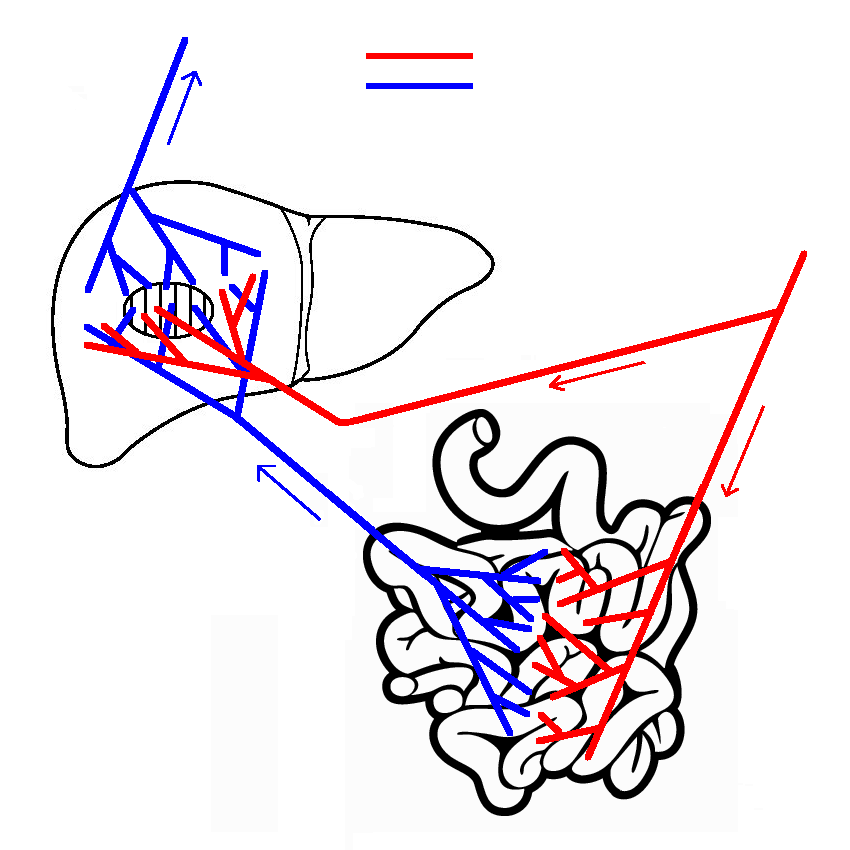
\includegraphics[width=100\unitlength]{schema/schema_irrigation_foie.png}}

%%% Cadre bordure
%\put(0,0){\line(0,1){100}}\put(0,0){\line(1,0){100}}
%\put(100,0){\line(0,1){100}}\put(0,100){\line(1,0){100}}

\put(57,92.5){Sang artériel, riche en oxygène}
\put(57,89){Sang veineux, pauvre en oxygène}

\put(40,75){Foie}
\put(82,18){Intestin grêle}
\put(82,15){et autres}
\put(83,12){organes du}
\put(82,9){tube digestif }

\linethickness{0.4\unitlength}
\put(18,65){\line(-10,-30){10}}
\put(1,32){Métastase}
\put(1,29){hépatique}

\put(57,56){ \begin{turn}{15} Artère hépatique \end{turn} }
\put(11,78){ \begin{turn}{70} Veine hépatique \end{turn} }
\put(31,49){ \begin{turn}{-40} Veine porte \end{turn} }
\put(77.5,48){ \begin{turn}{66} Artère \end{turn} }
\put(79,44){ \begin{turn}{66} mésentérique \end{turn} }
\end{picture}

\vspace{-10mm}
\caption{\label{fig:schema_irrig_foie} Schéma de l'irrigation du foie.}
\end{figure}

Pour réaliser ce type d'examen, on procède comme pour un simple scanner avec le même équipement. La différence réside dans l'injection en intraveineuse d'un produit de contraste iodé (PCI), juste avant l'examen. L'iode ayant un fort taux absorption  des rayons~X, il va éclaircir l'ensemble des zones dans lequel il se trouve. En ce qui concerne le foie, pour comprendre pourquoi le foie sain est plus éclaircit par le PCI que les métastases, nous devons nous intéressé à la manière dont arrive le PCI au foie et à la tumeur. La Figure~\ref{fig:schema_irrig_foie} présente le schéma général de la vascularisation du foie. Le foie possède une double vascularisation. La première est apportée directement depuis le coeur par l'artère hépatique. Du sang riche en nutriments (glucose et oygène) vient ainsi irriguer les cellules hépatiques? La seconde provient d'une dérivation. Le sang veineux en provenance du système digestif ne retourne pas directement au coeur~: il est envoyé au foie par la veine porte. Ce sang bien qu'étant pauvre en oxygène, est riche en glucose puisqu'il contient l'ensemble des éléments digérés. Dans un foie sain, la vascularisation portale est de l'ordre 70\% et la vascularisation artérielle de l'ordre de 30\%. Dans une tumeur hépatique, ce ratio est inversé~! REFF\todo{ref} En effet, en grandissant la tumeur va accroître ces besoins en glucose mais aussi en oxygène~: la néovascularisation se fait donc principalement depuis la vascularisation artérielle. 


Revenons au PCI. Dans la mesure où il y a deux voies sanguine pour accéder au foie, il y a deux temps caractéristiques~:
\begin{itemize}
\item Le \emph{temps artériel.} C'est le temps après l'injection, que le PCI met pour parvenir au foie par la voie artérielle. Il est d'environ 30 secondes. 
\item Le \emph{temps portal.} C'est le temps après l'injection, que le PCI met pour parvenir au foie par la voie portale. Il est d'environ 70 secondes. 
\end{itemize}
Les scanners réalisés avec PCI, sont effectué au temps portal. Ainsi au moment de l'acquisition de l'image, le PCI se trouve majoritairement dans les tissus vascularisées par la voie portale \ie le foie sain. Le tissu tumoral, beaucoup moins irriguer par voie portal contiendra donc nettement moins de PCI. Ceci se traduit directement sur le contraste de l'image médicale~: le tissu sain ayant fortement éclaircit, le tissu tumoral apparait de manière beaucoup plus évidente, en sombre. On pourra même distinguer des nuances au sein même de la tumeur (entre le centre et le pourtour notamment), ce qui va particulièrement nous intéressé pour tout ce qui concerne l'\hetero tumorale. L'ensemble des scanners présenté dans cet ouvrage a été réalisé avec un PCI.
\end{document}